% Phụ trách: B + C
% Nhiệm vụ: Xây dựng baseline — (Optional) SVM or Naive Bayes

\subsection{SVM}\label{subsubsec:svm-naive-bayes}

\subsubsection{Cơ sở lý thuyết}

\paragraph{1. Siêu phẳng phân tách và Bộ phân lớp lề cực đại}\mbox{}\\
Xét tập dữ liệu huấn luyện gồm $N$ mẫu $\{(\mathbf{x}_n, t_n)\}_{n=1}^{N}$, trong đó $\mathbf{x}_n \in \mathbb{R}^D$ là vector đặc trưng đầu vào và nhãn nhị phân $t_n \in \{-1, +1\}$ đại diện lần lượt cho hai lớp $\mathcal{C}_0$ (bình thường) và $\mathcal{C}_1$ (gian lận). Thông qua ánh xạ đặc trưng $\phi(\cdot)$ sang không gian nhiều chiều hơn, SVM tìm một siêu phẳng phân tách tuyến tính $y(\mathbf{x}) = \mathbf{w}^T \phi(\mathbf{x}) + b = 0$ sao cho khoảng cách từ siêu phẳng tới các điểm dữ liệu gần nhất của hai lớp (gọi là \textit{lề} -- margin, có độ rộng $\frac{2}{\|\mathbf{w}\|}$) đạt giá trị lớn nhất nhằm tối ưu khả năng tổng quát hóa (Hình~\ref{fig:svm-max-margin}).

\begin{figure}[H]
    \centering
    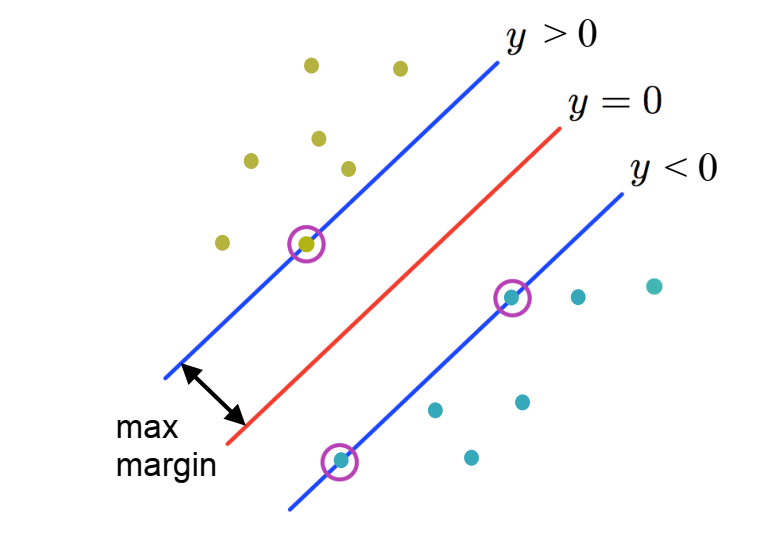
\includegraphics[width=0.72\linewidth]{graphics/svm_max_margin.png}
    \caption{Minh họa siêu phẳng phân tách lề cực đại và các vector hỗ trợ}
    \label{fig:svm-max-margin}
\end{figure}

\paragraph{2. SVM lề mềm và Bài toán đối ngẫu Lagrange}\mbox{}\\
Với dữ liệu thực tế có nhiễu và chồng lấp giữa hai lớp, mô hình bổ sung các biến bù $\xi_n \ge 0$ để cho phép một số điểm vi phạm ranh giới lề như minh họa tại Hình~\ref{fig:svm-soft-margin}. Bài toán tối ưu gốc của Soft-Margin SVM được phát biểu như sau:
\begin{equation}
    \min_{\mathbf{w}, b, \boldsymbol{\xi}} \; \frac{1}{2}\|\mathbf{w}\|^2 + C \sum_{n=1}^{N} \xi_n \qquad \text{với ràng buộc } \begin{cases} t_n\left(\mathbf{w}^T \phi(\mathbf{x}_n) + b\right) \ge 1 - \xi_n \\ \xi_n \ge 0 \end{cases}, \; \forall n = 1, \dots, N
\end{equation}
trong đó $C > 0$ là tham số điều chuẩn kiểm soát sự đánh đổi giữa việc mở rộng lề và mức phạt các điểm vi phạm.

\begin{figure}[H]
    \centering
    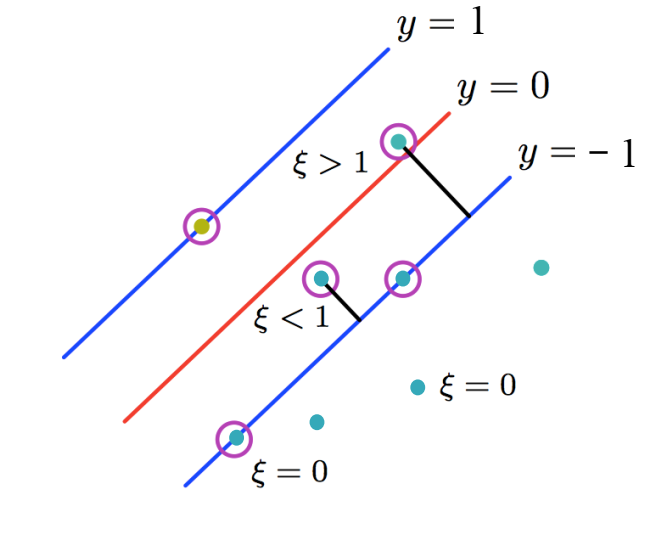
\includegraphics[width=0.72\linewidth]{graphics/svm_soft_margin.png}
    \caption{Cơ chế Soft-Margin SVM với các trường hợp giá trị của biến bù $\xi_n$}
    \label{fig:svm-soft-margin}
\end{figure}

Sử dụng nhân tử Lagrange $a_n \ge 0$, bài toán được chuyển sang dạng đối ngẫu:
\begin{equation}
    \max_{\mathbf{a}} \; \tilde{L}(\mathbf{a}) = \sum_{n=1}^{N} a_n - \frac{1}{2} \sum_{n=1}^{N} \sum_{m=1}^{N} a_n a_m t_n t_m K(\mathbf{x}_n, \mathbf{x}_m)
\end{equation}
thỏa mãn $0 \le a_n \le C$ và $\sum_{n=1}^{N} a_n t_n = 0$. Nhờ tính chất thưa (\textit{sparsity}), chỉ các điểm nằm trên hoặc vi phạm biên lề mới có $a_n > 0$ và được gọi là các \textbf{vector hỗ trợ} (tập $\mathcal{S}$), các điểm còn lại đều có $a_n = 0$. Hàm quyết định phân lớp khi đó chỉ phụ thuộc vào tập $\mathcal{S}$:
\begin{equation}
    y(\mathbf{x}) = \sum_{n \in \mathcal{S}} a_n t_n K(\mathbf{x}_n, \mathbf{x}) + b, \qquad \hat{t} = \text{sign}\big(y(\mathbf{x})\big)
\end{equation}

\paragraph{3. Kernel Trick và Hạt nhân RBF}\mbox{}\\
Thay vì tính tường minh tọa độ $\phi(\mathbf{x})$ trong không gian số chiều lớn (Hình~\ref{fig:svm-kernel-trick}), thủ thuật hạt nhân tính trực tiếp tích vô hướng thông qua hàm hạt nhân $K(\mathbf{x}_n, \mathbf{x}_m) = \phi(\mathbf{x}_n)^T \phi(\mathbf{x}_m)$. Với hạt nhân \textbf{RBF (Radial Basis Function / Gaussian)}, mức độ tương đồng giữa hai điểm dữ liệu được đo bằng khoảng cách Euclid:
\begin{equation}
    K_{\text{rbf}}(\mathbf{x}_n, \mathbf{x}_m) = \exp\left(-\gamma \|\mathbf{x}_n - \mathbf{x}_m\|^2\right)
\end{equation}
trong đó $\gamma > 0$ điều khiển độ rộng của phân phối Gaussian, kết hợp cùng tham số $C$ để định hình độ phức tạp của ranh giới quyết định phi tuyến (Hình~\ref{fig:svm-rbf-params}).

\begin{figure}[H]
    \centering
    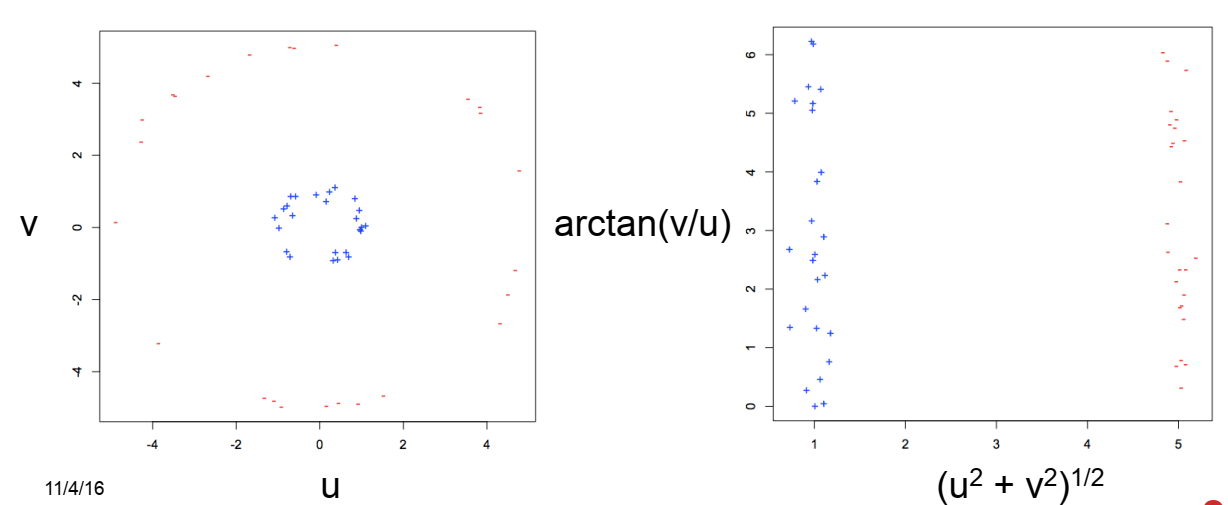
\includegraphics[width=0.82\linewidth]{graphics/svm_kernel_mapping.png}
    \caption{Ánh xạ dữ liệu không tách tuyến tính từ không gian gốc sang không gian đặc trưng chiều cao qua hàm $\phi(\mathbf{x})$}
    \label{fig:svm-kernel-trick}
\end{figure}

\begin{figure}[H]
    \centering
    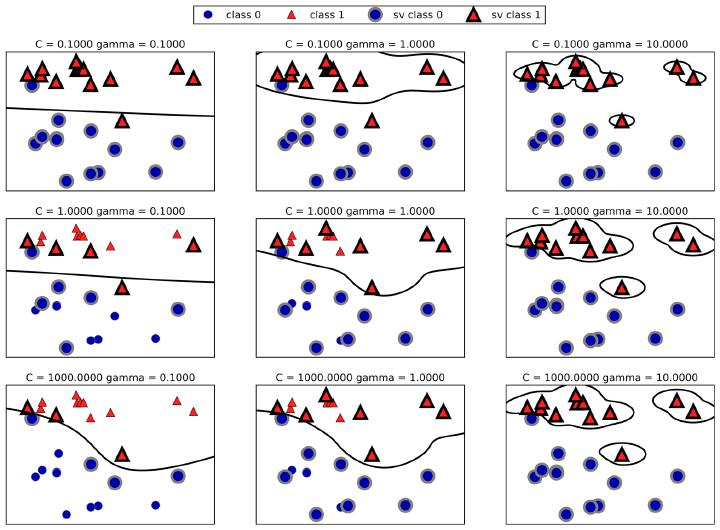
\includegraphics[width=0.85\linewidth]{graphics/svm_rbf_params.png}
    \caption{Ảnh hưởng của tham số điều chuẩn $C$ và độ rộng hạt nhân $\gamma$ lên ranh giới quyết định của RBF SVM}
    \label{fig:svm-rbf-params}
\end{figure}

\paragraph{4. Hiệu chỉnh xác suất hậu nghiệm (Platt Scaling)}\mbox{}\\
Do SVM thuần túy chỉ xuất giá trị khoảng cách có dấu $y(\mathbf{x})$ thay vì xác suất trực tiếp, kỹ thuật \textbf{Platt Scaling} được áp dụng bằng cách khớp một hàm Sigmoid lên đầu ra $y(\mathbf{x})$ thông qua kiểm định chéo nội bộ để ước lượng xác suất hậu nghiệm thuộc lớp gian lận $\mathcal{C}_1$:
\begin{equation}
    \hat{y} \triangleq p(\mathcal{C}_1 \mid \mathbf{x}) = \frac{1}{1 + \exp\big(A \, y(\mathbf{x}) + B\big)}
\end{equation}
với hai tham số vô hướng $A, B \in \mathbb{R}$ được tối ưu theo nguyên lý hợp lý cực đại trên các dự đoán ngoài \textit{fold}.

\subsubsection{Áp dụng mô hình vào bài toán}

\paragraph{1. Môi trường và Thư viện sử dụng}\mbox{}\\
Mô hình được triển khai bằng ngôn ngữ \textbf{Python} với các thư viện chính:
\begin{itemize}
    \item \texttt{scikit-learn}: Cung cấp bộ phân lớp \texttt{SVC}, \texttt{CalibratedClassifierCV} để hiệu chỉnh xác suất, \texttt{Pipeline} đóng gói luồng xử lý cùng hai bộ chuẩn hóa \texttt{RobustScaler} và \texttt{StandardScaler}.
    \item \texttt{imbalanced-learn}: Cung cấp kỹ thuật giảm mẫu ngẫu nhiên \texttt{RandomUnderSampler}.
    \item \texttt{NumPy}: Xử lý mảng và tính toán vector hóa.
\end{itemize}

\paragraph{2. Quy trình tiền xử lý, Cân bằng dữ liệu và Huấn luyện}\mbox{}\\
Quy trình thực nghiệm trong tệp \texttt{src/model\_b\_2.py} được thiết kế chặt chẽ nhằm ngăn ngừa rò rỉ dữ liệu (\textit{data leakage}) và tối ưu hóa độ phức tạp tính toán của Kernel SVM:
\begin{enumerate}
    \item \textbf{Chia dữ liệu phân tầng:} Dữ liệu sau làm sạch được tách thành tập huấn luyện toàn phần và tập kiểm tra độc lập, kết hợp kiểm định chéo \textit{Stratified K-Fold} để duy trì tỷ lệ lớp gian lận trên từng \textit{fold}.
    \item \textbf{Chuẩn hóa dữ liệu hai bước:} Do hạt nhân RBF dựa trên khoảng cách Euclid $\|\mathbf{x}_n - \mathbf{x}_m\|^2$ nên rất nhạy với chênh lệch thang đo giữa các chiều đặc trưng. Trong từng \textit{fold}, các cột số (\texttt{COLS\_TO\_SCALE}) trước tiên được chuẩn hóa bằng \texttt{RobustScaler} để triệt tiêu ảnh hưởng của ngoại lai, sau đó toàn bộ đặc trưng đi qua \texttt{StandardScaler} ($x'' = \frac{x' - \mu}{\sigma}$) bên trong \texttt{Pipeline} để đưa về trung bình $0$ và phương sai đơn vị.
    \item \textbf{Giảm mẫu lớp đa số trên tập huấn luyện:} Vì độ phức tạp huấn luyện của Kernel SVM tăng theo cấp số nhân với số lượng mẫu ($O(N^2)$ đến $O(N^3)$), kỹ thuật \texttt{RandomUnderSampler} với \texttt{sampling\_strategy=0.05} được áp dụng riêng trên tập huấn luyện con. Bước này giữ nguyên $100\%$ mẫu gian lận ($\mathcal{C}_1$) và lấy mẫu ngẫu nhiên lớp bình thường ($\mathcal{C}_0$) theo tỷ lệ $20:1$, trong khi tập kiểm định và tập kiểm tra giữ nguyên phân phối thực tế.
    \item \textbf{Hiệu chỉnh xác suất và Đánh giá:} Mô hình \texttt{SVC} được bọc trong \texttt{CalibratedClassifierCV} (\texttt{cv=5}, \texttt{method="sigmoid"}) để xuất xác suất dự đoán trên tập kiểm tra với ngưỡng phân loại $\lambda = 0.5$ và đánh giá qua mô-đun \texttt{src/metric\_model\_b\_2.py}.
\end{enumerate}

\paragraph{3. Thiết lập siêu tham số}\mbox{}\\
Cấu hình các siêu tham số cốt lõi trong hàm \texttt{handle\_imbalance()} và \texttt{build\_model()} được tổng hợp tại Bảng~\ref{tab:svm_hyperparams}.

\begin{table}[H]
\centering
\caption{Thiết lập siêu tham số cho mô hình Kernel SVM (\texttt{src/model\_b\_2.py})}
\label{tab:svm_hyperparams}
\renewcommand{\arraystretch}{1.2}
\begin{tabular}{|l|l|p{8.0cm}|}
\hline
\textbf{Thành phần / Tham số} & \textbf{Giá trị} & \textbf{Mục đích sử dụng} \\
\hline
\texttt{sampling\_strategy} & \texttt{0.05} & Giữ toàn bộ lớp gian lận và giảm mẫu lớp bình thường về tỷ lệ $20:1$, giảm chi phí tính toán và hạn chế thiên lệch. \\
\hline
\texttt{kernel} & \texttt{"rbf"} & Sử dụng hạt nhân Gaussian RBF để ánh xạ dữ liệu sang không gian phi tuyến chiều cao. \\
\hline
\texttt{C} & \texttt{2.0} & Tham số phạt biến bù của Soft-Margin SVM, tăng nhẹ độ chặt của ranh giới phân tách so với mặc định. \\
\hline
\texttt{gamma} & \texttt{"scale"} & Tự động tính $\gamma = \frac{1}{D \cdot \text{Var}(\mathbf{X})}$, điều chỉnh độ rộng hạt nhân thích ứng với phương sai dữ liệu. \\
\hline
\texttt{CalibratedClassifierCV} & \texttt{cv=5, sigmoid} & Thực hiện Platt Scaling qua kiểm định chéo 5-fold (\texttt{ensemble=False}) để hiệu chỉnh đầu ra thành xác suất tin cậy. \\
\hline
\texttt{random\_state} & \texttt{RANDOM\_STATE} & Cố định hạt giống ngẫu nhiên cho cả bộ giảm mẫu và mô hình SVC nhằm đảm bảo tính tái lập. \\
\hline
\end{tabular}
\end{table}